	\setlength{\tabcolsep}{3pt}
	\null\vfill\null
	\begin{center}
	\parbox{\textwidth-2\tabcolsep}{
		\begin{center}
			$\left.\begin{array}{cl} \text{10.\,Ky\={u}} & \raisebox{-7.2pt}{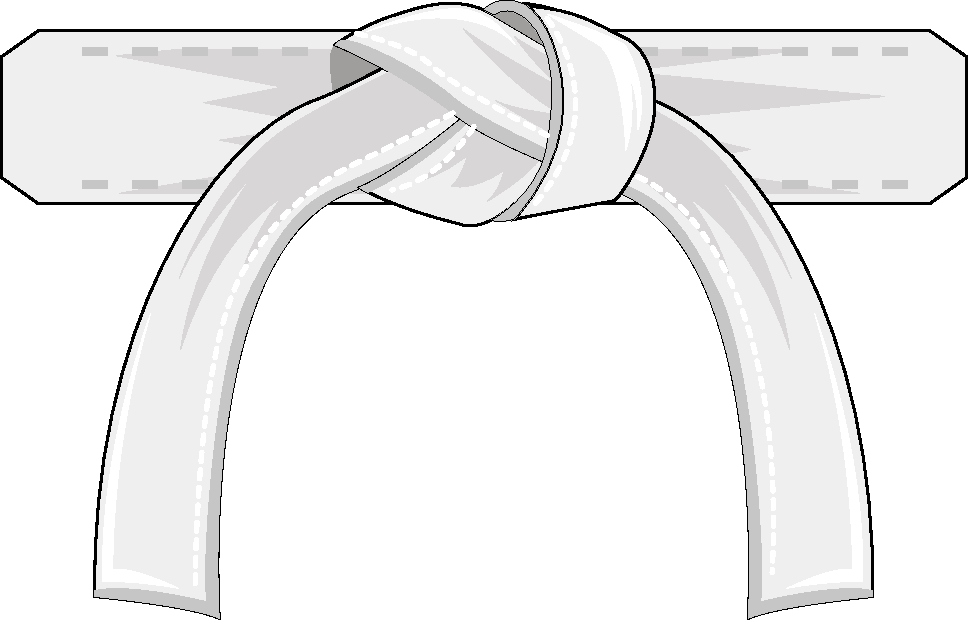
\includegraphics[height=24pt]{Gfx/gurte/whitebelt}}\\ \text{9.\,Ky\={u}} & \raisebox{-7.2pt}{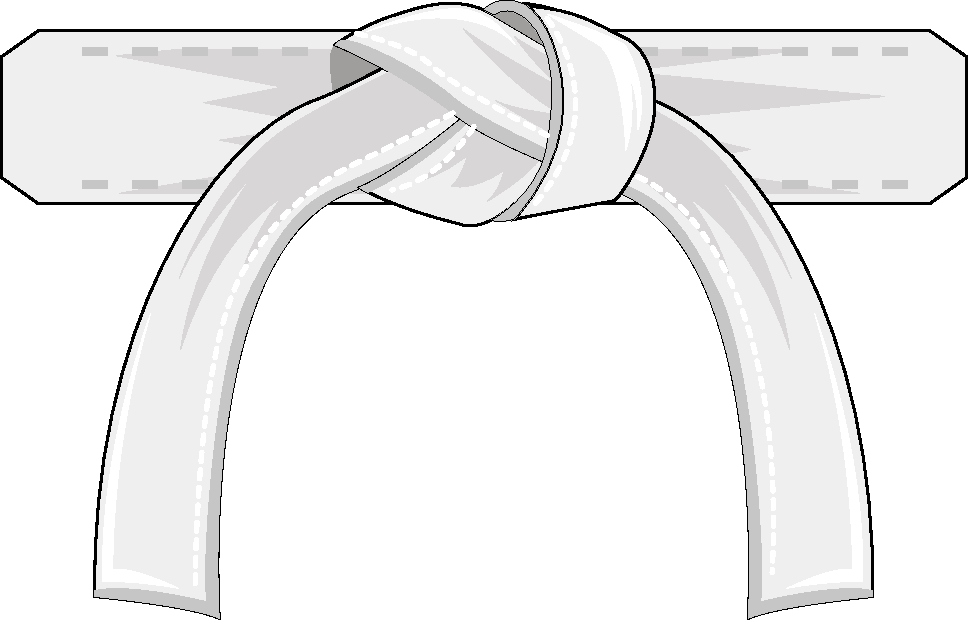
\includegraphics[height=24pt]{Gfx/gurte/whitebelt}}\\ \text{8.\,Ky\={u}} & \raisebox{-7.2pt}{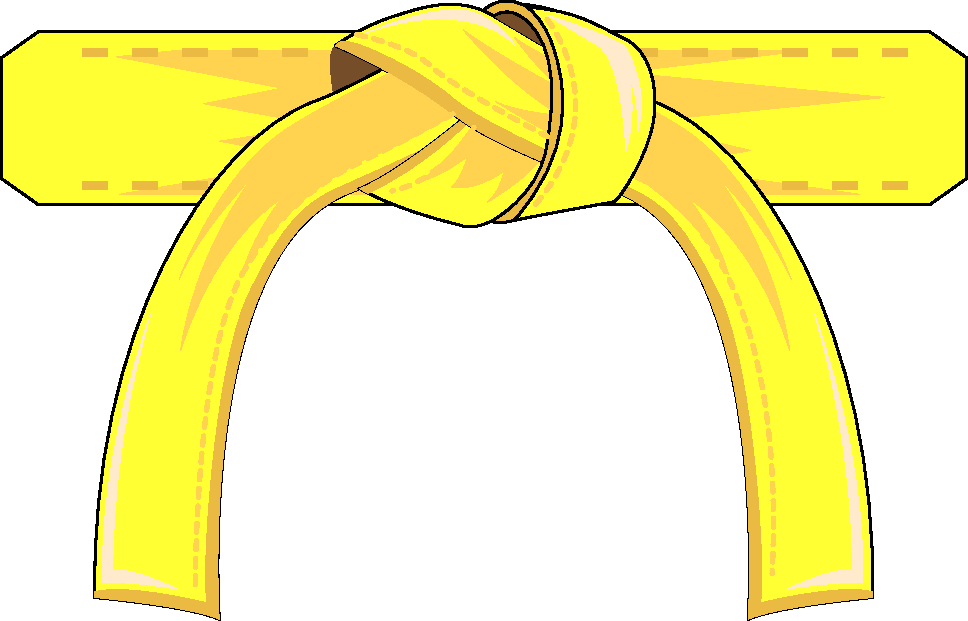
\includegraphics[height=24pt]{Gfx/gurte/yellowbelt}}\\ \text{7.\,Ky\={u}}& \raisebox{-7.2pt}{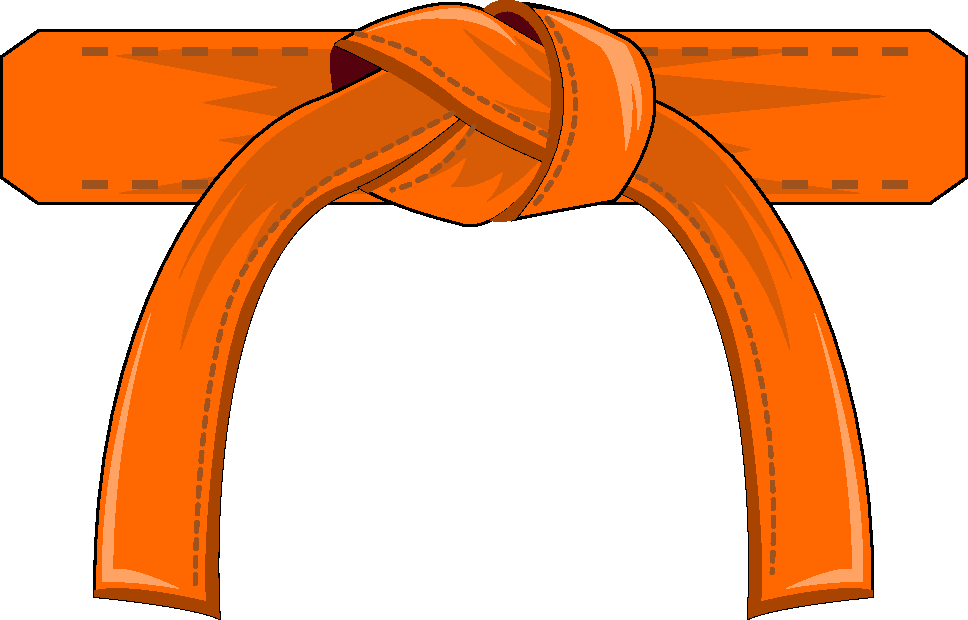
\includegraphics[height=24pt]{Gfx/gurte/orangebelt}}\end{array} \right\}\text{Unterstufe}$\quad$\left.\begin{array}{cl} \text{6.\,Ky\={u}} & \raisebox{-7.2pt}{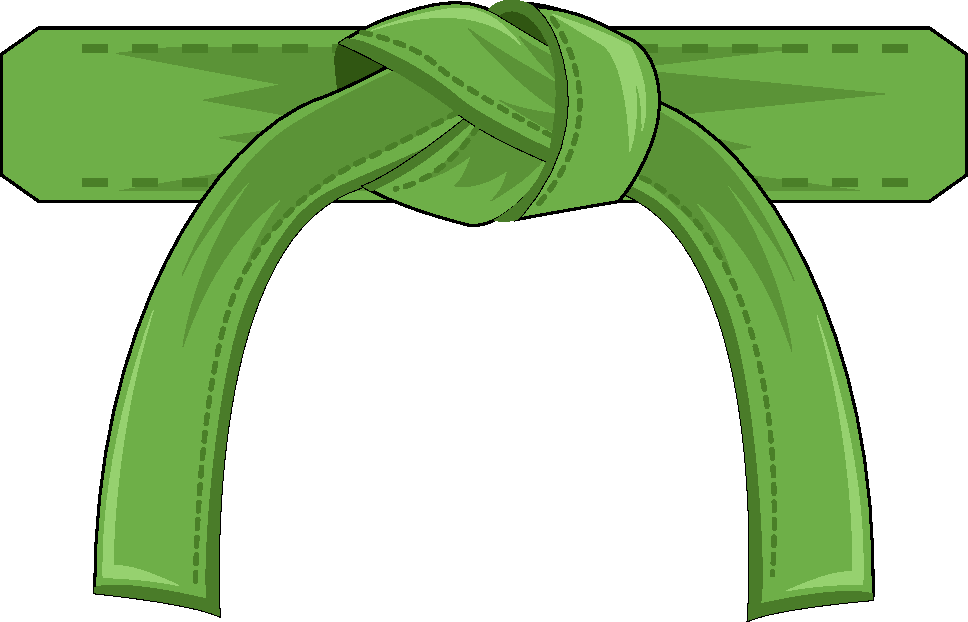
\includegraphics[height=24pt]{Gfx/gurte/greenbelt}} \\ \text{5.\,Ky\={u}} & \raisebox{-7.2pt}{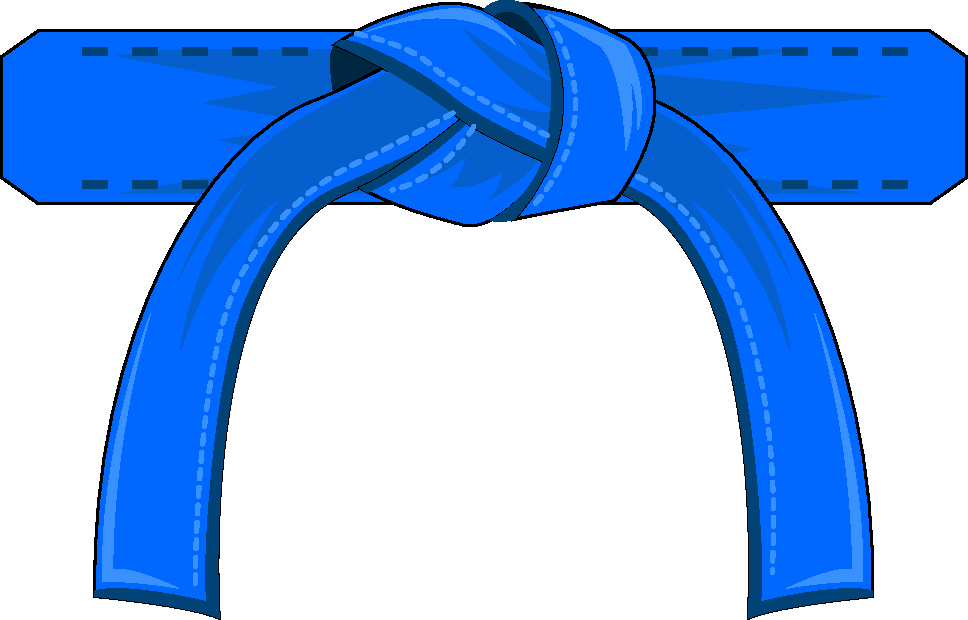
\includegraphics[height=24pt]{Gfx/gurte/bluebelt}}\\ \text{4.\,Ky\={u}} & \raisebox{-7.2pt}{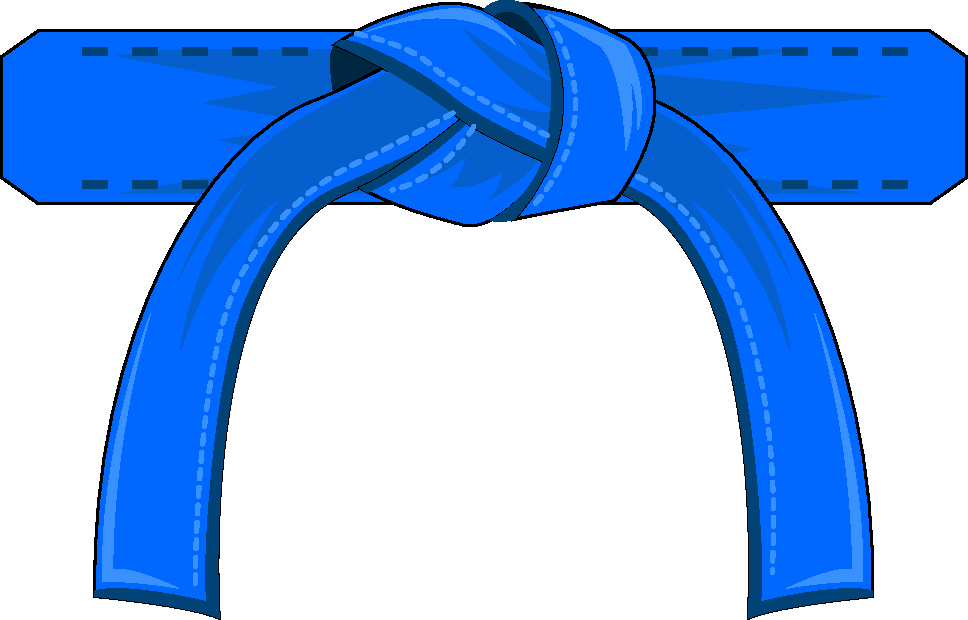
\includegraphics[height=24pt]{Gfx/gurte/bluebelt}}\end{array} \right\}\text{Mittelstufe}$\quad$\left.\begin{array}{cl} \text{3.\,Kyu} & \raisebox{-7.2pt}{
\includegraphics[height=24pt]{Gfx/gurte/brownbelt}}\\ \text{2.\,Ky\={u}} & \raisebox{-7.2pt}{
\includegraphics[height=24pt]{Gfx/gurte/brownbelt}} \\ \text{1.\,Ky\={u}} & \raisebox{-7.2pt}{
\includegraphics[height=24pt]{Gfx/gurte/brownbelt}}\end{array} \right\}\text{Oberstufe}$
		\end{center}
		Die Ky\={u}grade werden in unserem Dojo meist von unseren Trainern geprüft. Das jeweilige Prüfungsprogramm, sprich die zugrunde liegenden Techniken, Partnerformen, Kata sowie Kata-Bunkai, werden auf den entsprechenden Trainingskarten aufgelistet. \textit{\underline{Anmerkun}}g: zum 4.\,Ky\={u} wird bei uns \textit{nicht} auf einen \textit{violetten} Gürtel gewechselt, wir \textit{bleiben} auf \textit{blau}.\\

		Prüfungen finden meist 2\textit{x}\,pro Jahr statt. Der Trainingsfokus wird ca. 8 Wochen vor der Prüfung auf die jeweils geforderten Prüfungsinhalte gelegt. Je nach Anforderung werden dann innerhalb des Trainings entsprechende Gruppen gebildet, um eine gezielte Vorbereitung zu ermöglichen.\\

		\textit{Besonderheiten unseres Dojo:} Der Prüfungsinhalt zum 1.\,Kyu umfasst, zusätzlich zum eigentlichen Programm, auch die Inhalte der ebenfalls an diesem Tag stattfindenden Prüfungen - wenn zum Beispiel zur Prüfung zum 1.\,Kyu zwei Karateka angemeldet sind, sowie jeweils ein Karateka zum 9.,\,5.\,und 7.\,Kyu, so gehen die beiden zuerst genannten die jeweiligen Prüfungsprogramme der anderen ebenfalls mit - mit Ausnahme von Partnerformen und Kata-Bunkai. Findet an diesem Tag keine andere Prüfung statt, werden weitere Prüfinhalte im Vorfeld abgesprochen.
	}
	\end{center}\null\vfill\null
	\setlength{\tabcolsep}{6pt}